\documentclass[12pt,a4paper]{article}
\usepackage{geometry}
\usepackage{slashbox}
\geometry{
	a4paper,
	total={170mm,257mm},
	left=20mm,
	right=20mm,
	top=20mm,
	bottom=20mm
}
\usepackage{graphicx}
\usepackage{pdfpages}
\usepackage{placeins}
\usepackage{float}

\usepackage{polski}
\usepackage[utf8]{inputenc}

\begin{document}
	
	\begin{titlepage}
		\newgeometry{top=5.5cm, bottom=3cm}
		
		\centering
		{\huge\bfseries Logika układów cyfrowych lab.\par}
		
		\vspace{0.5cm}
		Prowadzący: Mgr inż. Antoni Sterna (E02-38m, wtorek 17:05) \\
	
		\vspace{1.1cm}
		{\Large sprawozdanie 9 - 2017.12.12\par}
		\vfill
		
		{\large\bfseries Jakub Dorda 235013\par}
		{\large\bfseries Marcin Kotas 235098\par}
		
		\vspace{1cm}
		\today \\ \LaTeX
		
		\restoregeometry
	\end{titlepage}

	\newgeometry{top=1.5cm, bottom=1.5cm, left=20mm, right=20mm}

	\section{Wprowadzenie/cel ćwiczeń}
	
		Celem ćwiczeń było zaprojektowanie automatu asynchronicznego statystycznego realizującego zadaną funkcję.
		Poznanie problemów występujących w tego typu układach oraz metod ich eliminacji; zjawiska hazardu i wyścigów.
		Po zaprojektowaniu układu oraz wyeliminowaniu niepożądanych zachowań, należało sprawdzić poprawność działania na
		zestawie UNILOG.
		
	\section{Tabela prawdy i siatki Karnaugh:}
		
		\subsection{Przebieg "czasowy" automatu:}
		
		\begin{table}[H]
			\centering
			\bgroup
			\setlength{\tabcolsep}{0.15cm}
			\begin{tabular}{r|ccccccccccccccccccccccccccccc}
					&	1	&	2	&	3	&	4	&	1	&	5	&	1	&	2	&	6	&	5	&	1	&	2	&	3	&	5	&	1	&	5	&	1	&	5	&	6	&	4	&	1	&	2	&	6	&	4	&	1	&	2	&	3	&	4	&	6	\\\hline
					$x_1$	&		&	-	&		&	-	&		&		&		&	-	&	-	&		&		&	-	&		&		&		&		&		&		&	-	&	-	&		&	-	&	-	&	-	&		&	-	&		&	-	&	-	\\
					$x_2$	&		&		&		&		&		&	-	&		&		&	-	&	-	&		&		&		&	-	&		&	-	&		&	-	&	-	&		&		&		&	-	&		&		&		&		&		&	-	\\
					y	&		&	-	&	-	&	-	&		&		&		&	-	&		&		&		&	-	&	-	&		&		&		&		&		&		&		&		&	-	&		&		&		&	-	&	-	&		&		\\
					
			\end{tabular}
			\caption{Uproszczony zapis przebiegu "czasowego" stanów automatu}
			\egroup
		\end{table}
			
			symbol "-" odpowiada stanowi wysokiemu, jego brak stanowi niskiemu
			
	
		\subsection{Tabele przejść/wyjść automatu:}
		
		\begin{table}[H]
			\begin{minipage}{.5\textwidth}
				\centering
				\begin{tabular}{c|c|c|c|c|c}
					\backslashbox{$Q$}{$x_1x_2$}	&	00	&	01	&	11	&	10	&  	Y 	\\\hline
					1	&	\textcircled{1}	&	5	&	-	&	2	&	0	\\\hline
					2	&	3	&	-	&	6	&	\textcircled{2}	&	1 \\\hline
					3	&	\textcircled{3}	&	5	&	-	&	4	&	1 \\\hline
					4	&	1	&	-	&	6	&	\textcircled{4}	&	0 \\\hline
					5	&	1	&	\textcircled{5}	&	6	&	-	&	0 \\\hline
					6	&	-	&	5	&	\textcircled{6}	&	4	&	0 \\	
				\end{tabular}
				\caption{tabela przejść/wyjść}
			\end{minipage}%
			\begin{minipage}{.5\textwidth}
				\centering
				\begin{tabular}{c|c|c|c|c|c}
					\backslashbox{$Q$}{$x_1x_2$}	&	00	&	01	&	11	&	10	&  	Y 	\\\hline
					1	&	\textcircled{1}	&	5	&	-	&	2	&	0	\\\hline
					2	&	3	&	-	&	6	&	\textcircled{2}	&	1 \\\hline
					3	&	\textcircled{3}	&	5	&	-	&	4	&	1 \\\hline
					4	&	1	&	\textcircled{4}	&	\textcircled{4}	&	\textcircled{4}	&	0 \\
				\end{tabular}
				\caption{po uproszczeniach}
			\end{minipage}
		\end{table}	
		
		\subsection{Kodowanie:}
		
			\begin{table}[H]
				\begin{minipage}{.5\textwidth}
					\centering
					\begin{tabular}{c|c|c|c|c}
						\backslashbox{$Q_1Q_2$}{$x_1x_2$}	&	00	&	01	&	11	&	10	\\\hline
						00	&	00	&	11	&	-	&	01	\\\hline
						01	&	10	&	-	&	11	&	\textcircled{01}	\\\hline
						10	&	\textcircled{10}	&	11	&	-	&	11 \\\hline
						11	&	00	&	\textcircled{11}	&	\textcircled{11}	&	\textcircled{11} \\
					\end{tabular}
					\caption{zakodowana tabela no.3}
				\end{minipage}%
				\begin{minipage}{.5\textwidth}
					\centering
					\begin{tabular}{c|c|c|c|c}
						\backslashbox{$Q_1Q_2$}{$x_1x_2$}	&	00	&	01	&	11	&	10	\\\hline
						00	&	00	&	10	&	10	&	01	\\\hline
						01	&	10	&	-	&	10	&	\textcircled{01}	\\\hline
						10	&	\textcircled{11}	&	10	&	10	&	10 \\\hline
						11	&	00	&	\textcircled{10}	&	\textcircled{10}	&	\textcircled{10} \\
					\end{tabular}
					\caption{kodowoanie po eliminacji wyścigów}
				\end{minipage}
			\end{table}	
			
			
			\begin{table}[H]
				\begin{minipage}{.5\textwidth}
					\centering
					\begin{tabular}{c|c|c|c|c}
						\backslashbox{$Q_1Q_2$}{$x_1x_2$}	&	00	&	01	&	11	&	10	\\\hline
						00	&	0	&	1	&	1	&	0	\\\hline
						01	&	1	&	-	&	1 	&	0	\\\hline
						11	&	1	&	1	&	1	&	1 	\\\hline
						10	&	0	&	1	&	1	&	1 	\\
					\end{tabular}
					\caption{$Q_1'$}
				\end{minipage}%
				\begin{minipage}{.5\textwidth}
					\centering
					\begin{tabular}{c|c|c|c|c}
						\backslashbox{$Q_1Q_2$}{$x_1x_2$}	&	00	&	01	&	11	&	10	\\\hline
						00	&	0	&	0	&	0	&	1	\\\hline
						01	&	1	&	-	&	0 	&	1	\\\hline
						11	&	1	&	0	&	0	&	0 	\\\hline
						10	&	0	&	0	&	0	&	0 	\\
					\end{tabular}
					\caption{$Q_2'$}
				\end{minipage}
			\end{table}	
		
			\begin{equation}
				\centering
				Q_1' = x_2 + \bar{x}_1 \cdot Q_2 + x_1 \cdot Q_1 = 
				\overline{\bar{x}_2 \cdot \overline{\bar{x}_1 Q_2} \cdot \overline{x_1 Q_1}}
			\end{equation}
			
			\begin{equation}
				\centering
				Q_2' = \bar{x}_1\bar{x}_2Q_2 + x_1\bar{x}_2\bar{Q}_1 + \bar{x}_2\bar{Q}_1Q_2 =
				\overline{\overline{\bar{x}_1\bar{x}_2Q_2} \cdot \overline{x_1\bar{x}_2\bar{Q}_1} \cdot 	\overline{\bar{x}_2\bar{Q}_1Q_2}}
			\end{equation}
			
			\begin{equation}
				\centering
				Y = Q_2'			
			\end{equation}
		
		\subsection{Użyte wzory:}
		
			\begin{equation}
			\overline{a\cdot b}=\bar{a}+\bar{b}
			\end{equation}
			\begin{equation}
			\overline{a+b}=\bar{a}\cdot\bar{b}
			\end{equation}
		
		\subsection{Schemat układu:}
		
		\begin{center}
			\makebox[\textwidth]{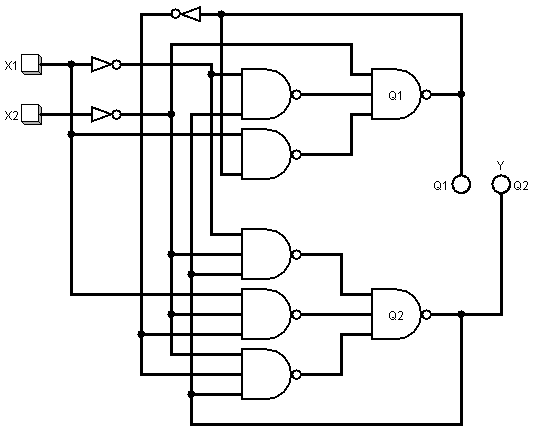
\includegraphics[width=\paperwidth - 75mm]{schem/circ.png}}
			Schemat 1 - automatu asynchroniczny
		\end{center}

	\section{Wnioski/podsumowanie}
	
			W celu sprawdzenia poprawności działania automatu asynchronicznego należało przeprowadzić testy dla wszystkich możliwych kombinacji wejść oraz stanów. Podczas testów należało też zbadać zachowanie układu w przypadku rozłączenia pętli zwrotnych.
	
\end{document}